\documentclass[ngerman]{article}
\usepackage[utf8]{inputenc}
%\usepackage[T1]{fontenc}
%\usepackage{lmodern}
\usepackage{amssymb,amsmath}
%\usepackage{ifxetex,ifluatex}
\usepackage{parskip}

\usepackage[german]{todonotes}
\usepackage{hyperref}
\hypersetup{colorlinks,linkcolor=,urlcolor=blue}

\usepackage{csquotes}
\usepackage{paracol}
\usepackage{listings}

\usepackage{enumitem}

\usepackage{float}
\newfloat{floatquote}{tbp}{loq}
\floatname{floatquote}{Zitat}
\usepackage{caption}
\captionsetup{font = small, format = hang}

% Um Zitate zu referenzieren
%\usepackage{cleveref}
%\crefname{floatquote}{Zitat}{Zitate}
%\Crefname{floatquote}{Zitat}{Zitate}

%\hypersetup{colorlinks=true,linkcolor=,urlcolor=black}
%\hypersetup{colorlinks=false}%,linkbordercolor=red,linkcolor=green}

\usepackage{algorithm}
\usepackage{algorithmic}

% Folgende Zeilen waren im orignalen Markdown Export, ich hab sie erstmal auskommentiert.
%\setlength{\parindent}{0pt}
%\setlength{\parskip}{6pt plus 2pt minus 1pt}
%\setlength{\emergencystretch}{3em}  % prevent overfull lines
%\setcounter{secnumdepth}{0}

\title{180: Testen, Verifizieren, Analysieren}
\author{Ricarda Schüler und Stefan Bunk}
\date{24.01.2016}


\begin{document}
\maketitle
\tableofcontents


\section{Überblick über die Anwendung}
\label{sec:ueberblick}

\paragraph{Sinn und Zweck}

180 ist eine Web-Anwendung, die Bachelor-Studenten des Hasso-Plattner-Instituts dabei unterstützt, eine korrekte Belegung zu finden, und somit ihr Bachelorstudium erfolgreich zu beenden.
Durch die Wahl von unterschiedlichen Vertiefungsgebieten sowie die Tatsache, dass viele Veranstaltungen mehreren Vertiefungsgebieten zuordenbar sind, kann es schwierig werden, eine korrekte Belegung zu finden.

Der Name 180 entstammt den 180 Leistungspunkten, die erforderlich sind, um das Bachelorstudium erfolgreich abzuschließen.
Es existiert desweiteren ein Schwesterprojekt namens 120, das von Masterstudenten des HPIs genutzt werden kann, und das den gleichen Zweck verfolgt.
Dieses Dokument befasst sich allerdings nur mit 180.

\paragraph{Entwicklungsparadigma und Programmiersprache}

Also typische Webanwendung wurde 180 in HTML, CSS und JavaScript geschrieben.
Dabei funktioniert es als rein clientseitige Anwendung, d.h. es benötigt keine weitere serverseitige Programmiersprache.
Es existieren keine automatisierten Tests, daher eignet sich das Projekt gut, um eine breite Testbasis in einem bestehenden Projekt aufzubauen.
Die Entwicklung folgt dem Wasserfallmodell.
Zunächst wurden die Anforderungen gesammelt, allerdings nicht formal, sondern in einer losen Liste.
Nach einer Planungsphase wurde das Projekt dann implementiert.
Nach der erfolgreichen Veröffentlichung ist das Projekt zurzeit in der Wartungsphase.

\paragraph{Anforderungen, Spezifikation und Dokumentation}

Die Anwendungen wurde aus dem persönlichen Bedarf heraus entwickelt, und es gab keinen externen Auftraggeber.
Alleiniger Entwickler war Stefan Bunk, einer der Autoren dieses Dokuments.
Obwohl es damit keine Spezifikation im klassischen Sinne gibt, sind dennoch die zu implementierenden Regeln genau festgelegt:
In der \href{http://www.uni-potsdam.de/ambek/ambek2010/15/Seite3.pdf}{Fachspezifischen Ordnung für das Bachelor- und Masterstudium im Fach IT-Systems Engineering an der Universität Potsdam}, der Studienordnung, wird genau festgelegt, wie ein Student seinen Belegungsplan zusammenstellen muss, um den Bachelorabschluss vom HPI zu erhalten.
Die Studienordnung wird in Abschnitt~\ref{sec:verification_and_validation} vorgestellt.

\paragraph{Aktueller Teststatus und Bug Repositories}

Wie bereits erwähnt existieren keine automatisierten Tests.
Bei der Enwicklung wurde der Code wiederholt manuell getestet.

Als \href{https://github.com/knub/onehundredandeighty/issues?q=is:issue}{Bug Repository} wird die von Github bereitgestellte Funktion der \emph{Issues} verwendet.
Dort kann der Entwickler, aber auch Nutzer der Anwender, Bug-Berichte oder Feature-Wünsche abgeben, die dann eine eindeutige Nummer erhalten.
Wurde der Fehler behoben, oder entschieden, den Wunsch nicht zu implementieren, kann das Issue geschlossen werden.

Bisher wurden fünf Issues gemeldet:
\begin{itemize}
    \item
        \href{https://github.com/knub/onehundredandeighty/issues/30}{2 Feature-Requests} nach Berechnung der Gesamtnote -- wird nicht implementiert
    \item
        \href{https://github.com/knub/onehundredandeighty/issues/20}{1 Syntaxfehler}, der die Ausführung des Programmes unmöglich machte
    \item
        \href{https://github.com/knub/onehundredandeighty/issues/4}{1 Feature-Request} nach variabler Anzahl der Semester, der teilweise umgesetzt wurde.
    \item
        \href{https://github.com/knub/onehundredandeighty/pull/5}{1 Issue} aufgrund einer Änderung der Wirtschaftsvorlesung, die statt zwei 3-LP-Veranstaltungen ab dem WS11/12 als eine 6-LP-Veranstaltung angeboten wurden.
\end{itemize}

\paragraph{Rollenverteilung der Tester}

Einer der Autoren dieses Dokumentes war der Entwickler von 180.
Beide Autoren sind bzw. waren in ihrem Bachelorstudium aktive Nutzer der Anwendung.
Im Folgenden werden beide auch noch die Rolle der Tester einnehmen.

\section{Initialer Test Plan}

\subsection{Verifikation und Validation}

\paragraph{Validation: Die richtige Anwendung bauen!}
\label{sec:verification_and_validation}

180 wurde entwickelt unter der Annahme, dass es für jeden Studenten kompliziert ist, sein Studium ent\-sprech\-end der Studienordnung zu planen.
Insbesondere die Beachtung aller Regeln der Vertiefungsgebiete ist kompliziert und erfordert mehrfaches Über\-prü\-fen aller Bedingungen.
Daher widmen wir uns dieser Regel auch in einem eigenen Abschnitt (\ref{sec:vertiefungsgebiete}).

%\begin{quote}
%    \begin{displayquote}
%        Das Bachelorstudium im Fach IT-Systems Engineering wird an der Universität Potsdam als Ein-Fach-Studium angeboten.
%        Es umfasst 180 LP inklusive Bachelorarbeit, Softwareprojekttätigkeit und 30 LP fachintegrativer Schlüsselqualifikationen.
%    \end{displayquote}
%    \captionof{floatquote}{Output of the Program}\label{quo1}
%\end{quote}

In diesem Bereich lässt die Studienordnung einen großen Spielraum zu, der entsprechend der eigenen Interessen ausgefüllt werden kann aber auch muss.
Die Menge aller gültigen Belegungen ist damit sehr groß, übersieht man allerdings eine einzige Bedingung führt dies zu einem ungültigen Belegungsplan.
Merkt man dies nicht rechtzeitig, muss im schlimmsten Fall ein weiteres Semester im Bachelorstudium eingeplant werden.

Daher ist die Idee von 180 diese manuelle und fehleranfällige Prüfung zu automatisieren.
Da die Regeln der Studienordnung sich nicht schnell ändern\footnote{Mehr zu möglichen Änderungen der Studienordnung im Abschnitt über die Sicherung der Qualität zukünftiger Releases, Abschnitt \ref{sec:releases}}, genügt es, die Regeln einmalig korrekt zu implementieren.
Daher ist dies auch der zentrale Punkt der Validierung:
Die Anwendung muss genau dann ausgeben, dass ein Belegungsplan valide ist, wenn er nach den Paragraphen der Studienordnung korrekt ist.
Kann die Anwendung dies nicht garantieren, ist sie nahezu nutzlos.
Wird der Anwendung nicht vertraut, wird sie niemand nutzen, da sowieso eine manuelle Prüfung notwendig wird.

Wir beginnen mit der Validation, indem wir jeden Paragraphen der Studienordnung analysieren, und daraus zu testende Eigenschaften eines korrekten Belegungsplans ableiten.
Sind aus einem Paragraphen keine Tests ableitbar, stellen wir dies in kursiver Schrift dar.

\setlength{\parindent}{0cm}

\begin{paracol}{2}
\textbf{§~1 Geltungsbereich}
\switchcolumn
\emph{Keine Tests notwendig, lediglich Einleitung}
\\
\switchcolumn*

\textbf{§~2 Gliederung des Studiums}
\switchcolumn
Es müssen mind. 180 LP erreicht werden.
\\
\switchcolumn*

\textbf{§~3 Dauer des Studiums}
\switchcolumn
Das Studium darf nicht länger als 12 Semester dauern.
\\
\switchcolumn*

\textbf{§~4 Nachteilsausgleich}
\switchcolumn
\emph{Keine Tests notwendig}
\\
\switchcolumn*

\textbf{§~5 Abschlussgrade}
\switchcolumn
\emph{Keine Tests notwendig, lediglich akad. Titel wird vorgestellt}
\\
\switchcolumn*

\textbf{§~6 Ziel des Studiums und Berufsrelevanz}
\switchcolumn
\emph{Keine Tests notwendig, lediglich Vision des Studiums}
\\
\switchcolumn*

\textbf{§~7 Studienverwaltung; Leis\-tungs\-er\-fas\-sungs\-pro\-zess}
\switchcolumn
\emph{Keine Tests notwendig, lediglich Information über Notenvergabe}
\\
\switchcolumn*

\textbf{§~8 Freiversuche}
\switchcolumn
Prüfungen dürfen maximal dreimal wie\-der\-holt werden.
\\
\switchcolumn*

\textbf{§~9(1) Module des Bachelorstudiums}
\switchcolumn
Die Veranstaltungen PT1, PT2, GDS, SWA, MOD1, MOD2, SWT1, Mathe1, Mathe2, TI1, TI2 müssen belegt werden.
Das gleiche gilt für die Veranstaltungen ``Wirtschaftliche Grundlagen'' und ``Rechtliche Grundlagen''.
\\
\switchcolumn*

\textbf{§~9(2) Softwarebasissysteme}
\switchcolumn
Die Veranstaltungen BS1 muss belegt werden.
Ebenso müssen von den  Veranstaltungen CG1, DBS1, POIS1, HCI1 sowie WWW mindestens drei belegt werden.
\\
\switchcolumn*

\textbf{§~9(3) Vertiefungsgebiete}
\switchcolumn
Dieser Paragraph beinhaltet die komplexen Regeln für Vertiefungsgebiete.
Dieser wird in Abschnitt \ref{sec:vertiefungsgebiete} behandelt.
\\
\switchcolumn*

\textbf{§~9(4) Softskills}
\switchcolumn
Die Veranstaltung ``Projektmanagement'' muss belegt werden.
Zusätzlich müssen 6 weitere LP im Gebiet Softskills belegt werden.
\\
\switchcolumn*

\textbf{§~10 Softskills}
\switchcolumn
\emph{Keine Tests notwendig, lediglich Information über Notenvergabe}
\\
\switchcolumn*

\textbf{§~11 Softwareprojekttätigkeit}
\switchcolumn
Das Bachelorprojekt muss im Umfang von 30 LP belegt werden.
\\
\switchcolumn*

\textbf{§~12 Bachelorarbeit}
\switchcolumn
Es muss eine Bachelorarbeit im Umfang von 12 LP geschrieben werden.
\\
\switchcolumn*

\textbf{§~13 -- §~19}
\switchcolumn
\emph{Keine weiteren Tests notwendig}
\\
\switchcolumn*
\end{paracol}

\paragraph{Verifikation: Die Anwendung richtig bauen!}

Um die Anwendung richtig zu bauen, folgt man der Spezifikation.
In diesem Fall gibt es keine interne, von den Entwicklern gemeinsam mit den Anwendern festgelegte Spezifikation.
Allerdings gibt es eine externe Spezifikation: die Studienordnung.
Diese wurde zwar nicht mit dem Ziel geschrieben, als Grundlage für die Entwicklung einer Anwendung zu stehen, doch definiert sie sehr genau die Anforderungen an einen korrekten Belegungsplan.
Wir betrachten daher im Folgenden die Studienordnung als die Spezifikation für 180.
Erfüllt 180 am Ende alle Paragraphen der Studienordnung mit im Programm implementierten Regeln, ist das Programm korrekt.

Die Studienordnung ist als Artefakt sehr statisch, sie ändert sich nahezu nie.
Zusätzlich zur Studienordnung sind aber die halbjährlich erscheinenden Vorlesungsverzeichnisse relevante Artefakte für 180.
In diesen wird festgelegt, welche Veranstaltungen angeboten werden und welchen Gebieten sie zugeordnet werden können.
Damit ist die Anwendung auch niemals fertig, da diese Pflege der Daten halbjährlich vorgenommen werden muss.

In unserem Fall reicht es, die Validation einmalig durchzuführen, da sich die Studienordnung nicht ändert.
Mit der Abdeckung aller Paragraphen ist sichergestellt, dass 180 auch wirklich den Anforderungen der Studenten genügt.
Die Verifikation, u.a. die korrekte Implementierung der Regeln sowie die korrekte Aktualisierung der Semesterdaten, muss permanent durchgeführt werden.
Dies geschieht auch im Rahmen dieses Projektes, indem wir Tests entwickeln.

\subsection{Welche Technologien sollen während der Entwicklung angewandt werden?}

180 ist ein abgeschlossenes Projekt für das bisher keine Tests existieren.
Insofern können keine Technologien oder Entwicklungsparadigmen wie TDD mehr während der Entwicklung angewandt werden.

Wir werden aber im folgenden einige Technologien vorstellen, die wir nun im Nachhinein anwenden werden, um 180 auf mögliche Fehler zu überprüfen.
Zu\-nächst sprechen wir dabei natürlich von Tests.
Wir werden uns dabei insbesondere auf Tests der Kern-Logik des Programms konzentrieren, also ob ein Belegungsplan valide ist oder nicht (und warum nicht).
Dabei werden im Rahmen dieses Dokuments auch Mutation Tests ausprobieren.
Dabei werden minimale Änderungen im Programm vorgenommen und geschaut, ob ein Test die entsprechende Änderung abfängt.
Wir denken, dies ist eine gute Möglichkeit um einzuschätzen, wie abdeckend unsere Tests sind.
Randomisiertes Testing bietet sich bei dem Projekt nicht an.
Die Testfälle, also konkrete Belegungspläne, müssen sehr genau ausspezifiziert sein, um bestimmte Grenzfälle abzudecken.
Eine zufällige Belegung wird nahezu immer nicht valide sein.

Statische Analyse kann ebenfalls helfen Bugs oder Unsauberkeiten im Programm zu finden.
Daher werden wir verschiedene Tools zur statischen Analyse in JavaScript ausprobieren.
Einer der oben erwähnten Issues wäre mit statischer Analyse zum Beispiel leicht zu entdecken gewesen.

% Laut dem ursprünglichen Paper von D. Hamlet über Random Testing.
% The [..] meaning of ``random testing'' refers to an
% explicit lack of ``system'' in the choice of test data, so that there is
% no correlation among different tests.

Beim Tradeoff zwischen Kosten und Korrektheit liegt bei uns der Fokus ganz klar auf der Korrektheit.
Die Korrektheit der implementierten Regeln ist oberstes Gut, weil eine fälschlicherweise korrekte Belegung schwere Konsequenzen für den jeweiligen Studenten haben kann, z.B. wenn ein Semester länger studiert werden muss.


\subsection{Wann ist die Anwendung bereit für eine Veröffentlichung?}

Wir definieren Fertigkeit (``readiness'') auf Basis von drei Faktoren:

\begin{itemize}
    \item \textbf{Korrektheit}:
        Wie bereits im ersten Abschnitt erwähnt ist die Korrektheit der Anwendung das wichtigste Kriterium.
        Alle Regeln der Studienordnung müssen korrekt implementiert und abgedeckt sein.
    \item \textbf{Vertraulichkeit}:
        Die Daten des Nutzers verbleiben immer auf dem lokalen Rechner und werden insbesondere nicht in einer Datenbank gespeichert.
        Der Belegungsplan eines Nutzers sollte privat bleiben und für den Betreiber des Servers niemals einsehbar sein.
    \item \textbf{Usability}:
        Die Webseite sollte gut zu benutzen sein.
        Insbesondere muss zu jedem Zeitpunkt klar sein, was die aktuelle Belegung ist, und ob diese korrekt ist oder nicht.
\end{itemize}

Von den drei Fertigkeits-Kriterien ist die Usability am schwierigsten zu erfassen, da dieses subjektive Empfinden nur über eine User-Study ermittelt werden kann.
Dies geschieht nicht im Rahmen dieses Projektes.
Bei der Vertraulichkeit geht es darum, dass wir sensibel mit den Daten des Nutzers.
Insbesondere ist wichtig, dass wir den Belegungsplan des Nutzers nicht auf dem Server speichern.
Dies erreichen wir, indem wir per Design die Daten nur auf dem Rechner des Nutzers speichern, und sie nie über das Netzwerk schicken.
Daher erfordert diese Anforderung keine expliziten Tests.

Die Korrektheit der Anwendung überprüfen wir im folgenden Kapitel ausführlich über automatisierte Tests sowie statische Analyse.
Das wir die richtigen Regeln implementieren, haben wir bereits im Abschnitt zur Validierung beschrieben.

Ein weiterer üblicherweise gewählter Faktor um die ``readiness'' zu definieren ist die Verlässlichkeit (``reliability'') der Anwendung.
Dies ist aber in unserem Fall kein Problem, weil es sich um eine statische Webseite handelt, und damit keinerlei Ressourcen des Server über das Ausliefern der Seite hinaus benötigt werden.
Desweiteren kann sich der Nutzer die Anwendung auch lokal auf seinen Rechner herunterladen, und die Anwendung so nutzen.
Selbst wenn der Nutzer auf die Online-Anwendung vertraut und diese für eine kurze Zeit nicht erreichbar ist, stellt dies auch kein Problem dar, da eine Studien- und Belegungsplanung üblicherweise über einen Zeitraum von mind. 3 Jahren erfolgt.

\subsection{Wie wird die Qualität in zukünftigen Releases sichergestellt?}
\label{sec:releases}

Das Hauptproblem der Aktualisierung sind die halbjährlich veröffentlichten Lehrveranstaltungsverzeichnisse.
Diese müssen manuell in 180 eingepflegt werden.
Listing~\ref{lst:data} zeigt einen Ausschnitt aus der Daten-Datei.
Hierbei ist insbesondere auf die Vertiefungsgebiete einer Veranstaltung zu achten.
Wird bei einer Veranstaltung ein falsches Vertiefungsgebiet eingetragen, macht dies eigentlich gültige Belegungen ungültig, oder erlaubt Belegungen, die nicht erlaubt werden sollten.

Da die Pflege dieser Daten manuell geschieht, ist sie sehr fehleranfällig.
In der Vergangenheit kam es bereits zu Fehlern in diesen Daten\footnote{Siehe z.B. \url{https://github.com/knub/onehundredandeighty/issues/20}}.
Solche Fälle durch Tests abzudecken ist kompliziert.

\begin{lstlisting}[caption=Ausschnitt aus \texttt{data.js},label={lst:data},frame=single]
/* .. weitere Veranstaltungen .. */
    swq: {
        kurz: "SW-Qualitaet",
        lehrform: ["Vorlesung", "Projekt"],
        modul: ["Vertiefungsgebiete"],
        semester: ["SS14", "WS15/16"],
        pflicht: false,
        empfohlen: "",
        vertiefung: ["OSIS", "SAMT"],
        cp: 6,
        vorher: [],
        dozent: ["Prof. Dr. Holger Giese"],
        nameLV: "Softwarequalitaet"
    },
/* .. weitere Veranstaltungen .. */
\end{lstlisting}


Ein offensichtliches Problem stellt die Änderung oder Neuverfassung der Studienordnung dar.
In diesem Fall muss die Anwendung entweder behutsam angepasst werden, oder komplett neu entwickelt werden.
Deswegen ist es wichtig, von einer Änderung der Studienordnung so schnell wie möglich zu erfahren.
Es lässt sich dafür aber keine gute technische Lösung implementieren.
Da Änderungen der Studienordnung aber öffentlich angekündigt werden müssen, und oft auch mit Diskussionen zwischen den Studierenden und Lehrenden einhergehen, verlassen wir uns auf schnelles Feedback des Fachschaftsrates oder der Studierendenschaft, auch wenn die Autoren selbst nicht mehr studieren werden.

Technologisch sind keine Inkompatibilitäten in den nächsten Jahren zu erwarten.
180 nutzt moderne Webtechnologien wie HTML5, CSS3 und JavaScript.
Deswegen ist in den nächsten Jahren keine Inkompatibiliät oder Beendigung der Unterstützung durch Browser-Hersteller zu erwarten.

\subsection{Wie kann der Entwicklungsprozess selbst verbessert werden?}

Wie bereits erwähnt ist das Hauptproblem die Aktualisierung der Veranstaltungsdatenbank.
Dabei kommt es desöfteren zu Fehlern.
Technisch gesehen ist eine Kontrolle hier schwierig.
Wenn eine neue Veranstaltung angeboten wird, ist nicht direkt zu erkennen, dass diese zum Beispiel fälscherlicherweise dem Vertiefungsgebiet BPET statt HCT zugeordnet wurde, oder das die Anzahl der Credit Points falsch ist.
Insofern ist dieses Problem nur durch die Einführung eines Korrekturprozesses möglich.
Zwei Ideen dafür wären:

\begin{itemize}
    \item Code Reviews: Jede Änderung an den Daten muss von mindestens zwei weiteren Personen manuell überprüft werden.
    \item Unabhängige Updates: Zwei Personen aktualisieren unabhängig voneinander die Veranstaltungsdatenbank. Erst wenn beide Updates semantisch identisch sind, werden die Änderungen in das System übernommen.
\end{itemize}

Geht man davon aus, dass eine solche Anwendung neu entwickelt wird, würden wir Test-Driven-Developments (TDD) vorschlagen. 
Dadurch würde jede Anforderung direkt mit einem Test geprüft und die Korrektheit der Anwendung sicher gestellt.
Wie bereits beschrieben ist, die Korrektheit der wichtigste Punkt in der Anwendung, so dass TDD die Validation und die Readiness der Anwendung aktiv unterstützt.

\subsection{Klassifizierung nach verschiedenen Test-Kriterien}

\paragraph{Validation- oder Defekt-Testen}
Unsere Tests lassen sich hauptsächlich der Kategorie Validation-Testing zuordnen, da wir immer von einen oder mehreren Paragraphen der Studienordnung ausgehen und schauen, ob dessen Anforderungen implementiert sind.
Dabei geschieht zwar implizit auch Defect-Testing, da die Tests ja auch fehlschlagen, wenn es einen Bug im System gibt, aber von der Sichtweise her betrachten wir Validation-Tests.

\paragraph{Unit-, Integration- und System-Testen}
Wir betrachten nur Unit- und Integrationstests.
Erstere betrachten wir, indem wir einzelne Regeln, wie z.B. ``ein Kurs kann nur in einem Semester belegt werden, in dem er angeboten wird'' testen.
Schlussendlich testen wir aber auch die Integration aller Regel-Komponenten, indem wir fertige Belegungspläne mit allen Regeln überprüfen.
Lediglich System-Testing werden bei uns nicht durchgeführt, da wir keine Front\-end-Tests schreiben und damit nicht das System dem User Interface testen.

\paragraph{Development-, Release- oder Usertesting}
Unsere Tests lassen sich als Development-Tests kategorisieren.
Spezielle Tests vor einem Deployment werden nicht durchgeführt, ebenso keine Tests mit echten Nutzern.

\subsection{Zusammenfassung}
\label{sec:zusammenfassung}

Im Folgenden fassen wir zusammen, wie wir den Status quo durch unseren initialen Test-Plan verbessern möchten.

\begin{itemize}
    \item Vollständiges Mapping zwischen Regeln und Paragraphen (dies wurde bereits in Kapitel~\ref{sec:verification_and_validation} gezeigt)
    \item
        Defekt-Testing: Durch statische Analyse erkennen, ob die Datei \texttt{data.js} Syntax-Fehler enthält
    \item
        Unit-Tests für jede Regel im Programm
    \item
        System-Tests mit kompletten, echten Belegungsplänen
\end{itemize}


\section{Testing}

In diesem Kapitel werden Beispiele für verschiedene Testarten dargestellt. Dabei wurde versucht die Anwendung in die breite hin zu testen. Das heißt für die verschiedenen Ansätze wurde jeweils eine Funktion von 180 ausgewählt. In den meisten Fällen gibt es weitere Programmteile, welche genau so getestet werden können. Es geht in diesem Abschnitt aber viel mehr darum, einen Überblick zu geben, was überhaupt möglich ist.
GUI-Testing haben wir in diesem Abschnitt erst einmal nicht betrachtet, sondern uns auf die Logik im Hintergrund konzentriert.

\subsection{Graph Coverage}

\subsubsection{Control Flow Graph}
Es gibt die sogenannte Time Rule.
Diese prüft, ob eine bestimmte Lehrveranstaltung in einem bestimmten Semester angeboten wurde beziehungsweise wahrscheinlich angeboten werden wird.
Der Algorithmus zur Prüfung ist in Pseudocode in Algorithmus \ref{algo:time_rule} dargestellt. Der daraus resultierende Graph ist in Abbildung \ref{fig:graph_time_rule} zu sehen.

\begin{algorithm}[h!]
\caption{Time Rule}
\label{algo:time_rule}
\algsetup{indent=2em}
\begin{algorithmic}[1]
    \REQUIRE 1 Course
    \ENSURE Boolean (offered in this semester)
    \STATE semester = getSemester(course)


    \IF{course chosen}
        \RETURN true
    \ELSE
        \IF{Semester is in past}
            \RETURN course offered in semester?
        \ELSE
            \IF{semester is Sommersemester}
                \RETURN course offered in this semester or offered in past sommersemester
            \ELSE
                \IF{semester is Wintersemester}
                    \RETURN course offered in this semester or offered in past Wintersemester
                \ELSE
                    \RETURN Error
                \ENDIF
            \ENDIF
       \ENDIF
   \ENDIF
\end{algorithmic}
\end{algorithm}


\begin{figure}[h!]
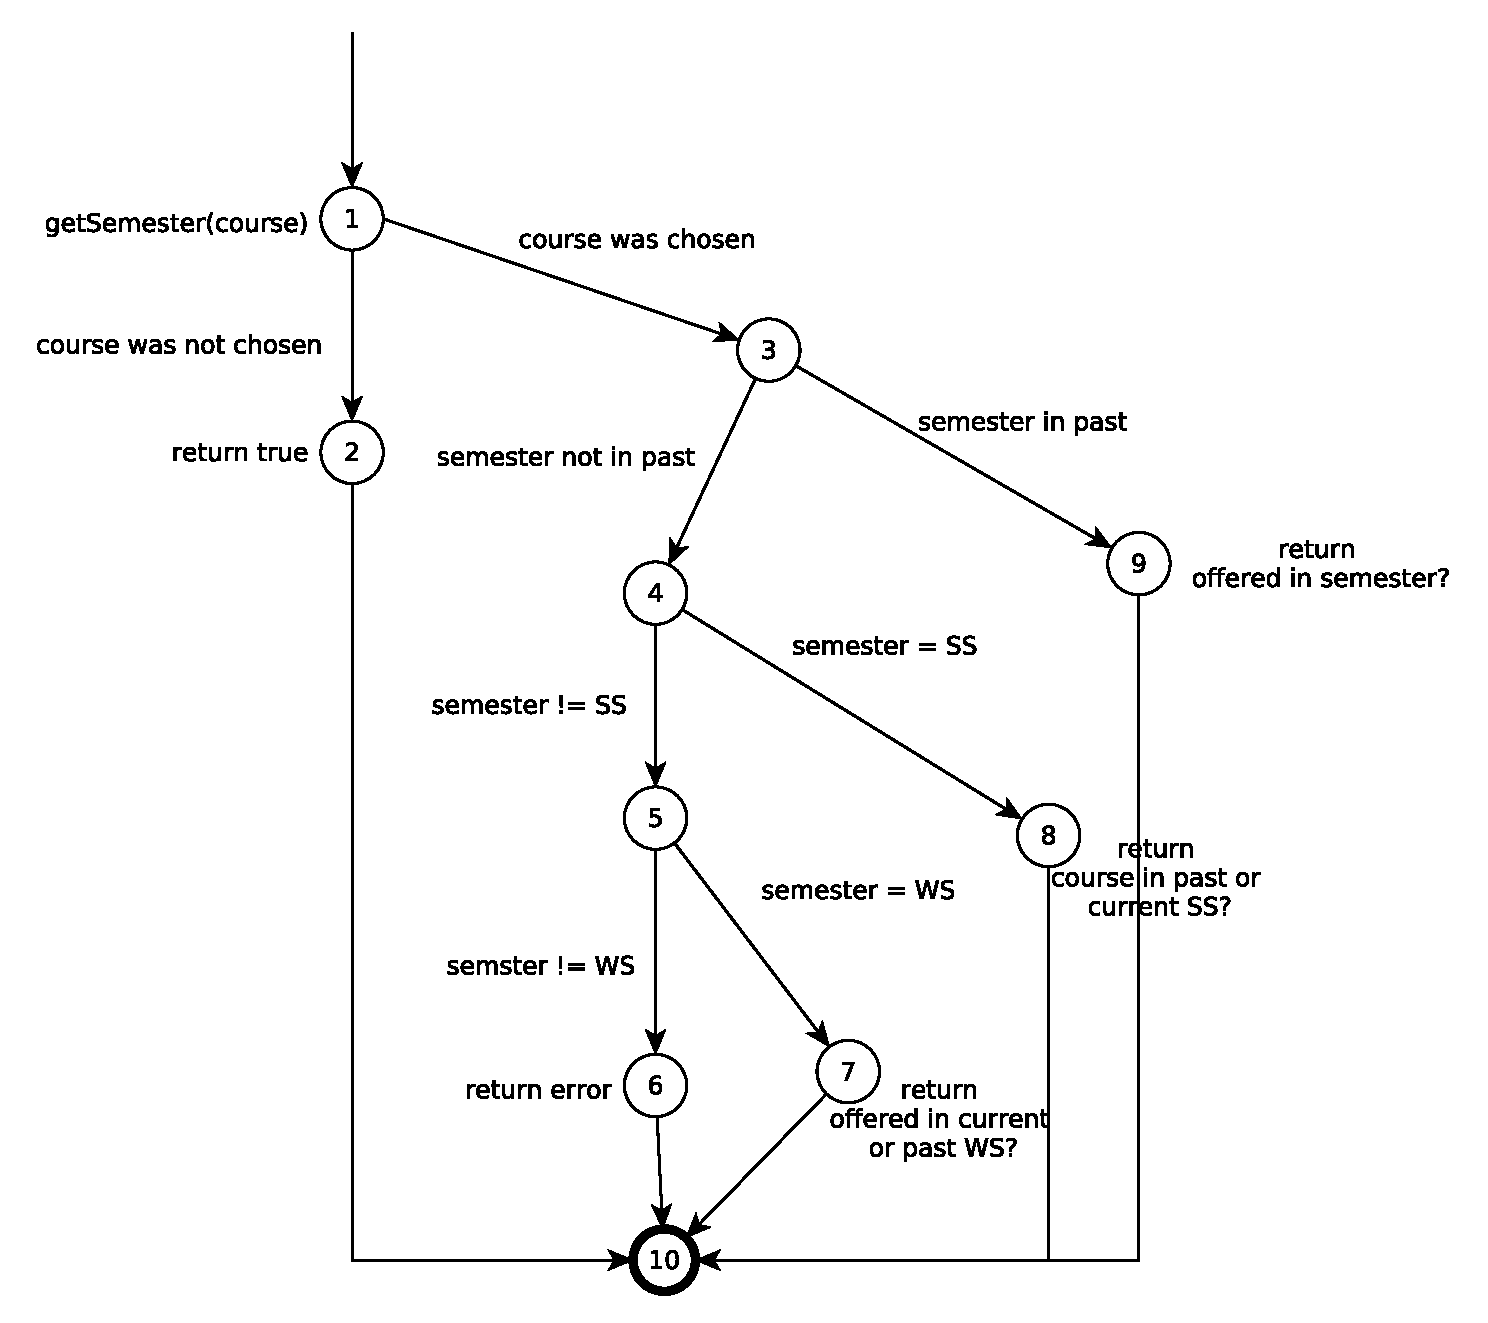
\includegraphics[width=0.8\textwidth]{figures/time_rule.pdf}
\caption{Graph der Time Rule}
\label{fig:graph_time_rule}
\end{figure}

Wir möchten Edge-Pair-Coverage für diese Regel erreichen, da damit alle Fälle abgedeckt sind.
Dazu müssen Kanten-Kanten-Kombinationen in der Testsuite enthalten sein.
Nachfolgend sind alle Test Requirements und Testpfade abgebildet. Die Testpfade, welche zusammen alle Fälle abdecken, wurden mit automatisierten Tests umgesetzt \footnote{Tests siehe \url{https://github.com/knub/onehundredandeighty/blob/testing/test/cfg_test.js}}.


\vspace{1em}


\begin{paracol}{2}
 \textbf{Test Requirement}
\begin{enumerate}[label=\Alph*]
\item $\lbrack 1,2,10 \rbrack$
\item $\lbrack 1,3,4\rbrack$
\item $\lbrack 1,3,9\rbrack$
\item $\lbrack 3,4,5\rbrack$
\item $\lbrack 3,4,8\rbrack$
\item $\lbrack 3,9,10\rbrack$
\item $\lbrack 4,5,6\rbrack$
\item $\lbrack 4,5,7\rbrack$
\item $\lbrack 4,8,10\rbrack$
\item $\lbrack 5,6,10\rbrack$
\item $\lbrack 5,7,10\rbrack$
\end{enumerate}

\switchcolumn
\paragraph{Test Paths}
\begin{enumerate}[label=(\roman*)]
\item $\lbrack 1, 2, 10 \rbrack$
\item $\lbrack 1, 3, 4, 5, 6, 10\rbrack$
\item $\lbrack 1, 3, 4, 5, 7, 10\rbrack$
\item $\lbrack 1, 3, 4, 8, 10\rbrack$
\item $\lbrack 1, 3, 9, 10\rbrack$
\end{enumerate}

\begin{table}
\begin{tabular}{|l|p{2.5cm}|}
\hline
\textbf{Test Pfade} & \textbf{Abgedeckte TR} \\ \hline \hline
(i) & A\\ \hline
(ii)  & B, D, G, J \\ \hline
(iii) & B, D, H, K\\ \hline
(iv) & B, E, I\\ \hline
(v) & C, F\\ \hline \hline
Coverage & A, B, C, D, E, F, G, H, I, J, K, H\\ \hline
\end{tabular}
\end{table}

\end{paracol}

Die Methode war sehr gut mit Control Flow Coverage testbar. Es gibt noch viele weitere logische Programmabschnitte, welche ähnlich aufgebaut sind und damit gut mit Control Flow Coverage die Testpfade und Requirements gefunden werden können. Allerdings ist diese Methode auch recht aufwendig durchzuführen. 

% \subsubsection{Finite State Machines}
% Veranstaltungsstatus: gewählt, wählbar, gefiltert...


\subsubsection{Use Cases}
Für \emph{onehundredandeighty} haben wir die folgenden Use Cases ermittelt:

\begin{itemize}
    \item Semester wählen
    \item Semesteranzahl verändern
    \item Belegung wählen
    \item Belegung validieren
    \item Filtern nach verfügbaren Kursen
\end{itemize}

Alle Use Cases sollten hinreichend getestet werden, allerdings haben wir uns im Rahmen des Seminares auf einen Use Case beschränkt.
Für eine genaue Prüfung haben wir uns den Use Case "Belegung wählen" heraus gesucht. Dieser Use Case ist ein sehr zentraler Bestandteil der Anwendung, welcher für den Nutzer eine relativ hohe Komplexität aufweist. In Abbildung \ref{fig:aktivity_belegung_waehlen} ist das Aktivitätsdiagram dargestellt. Dieses Aktivitätsdiagram interpretieren wir nun als Graph, welcher in Abbildung \ref{fig:graph_belegung_waehlen} dargestellt ist.

\begin{figure}[h!]
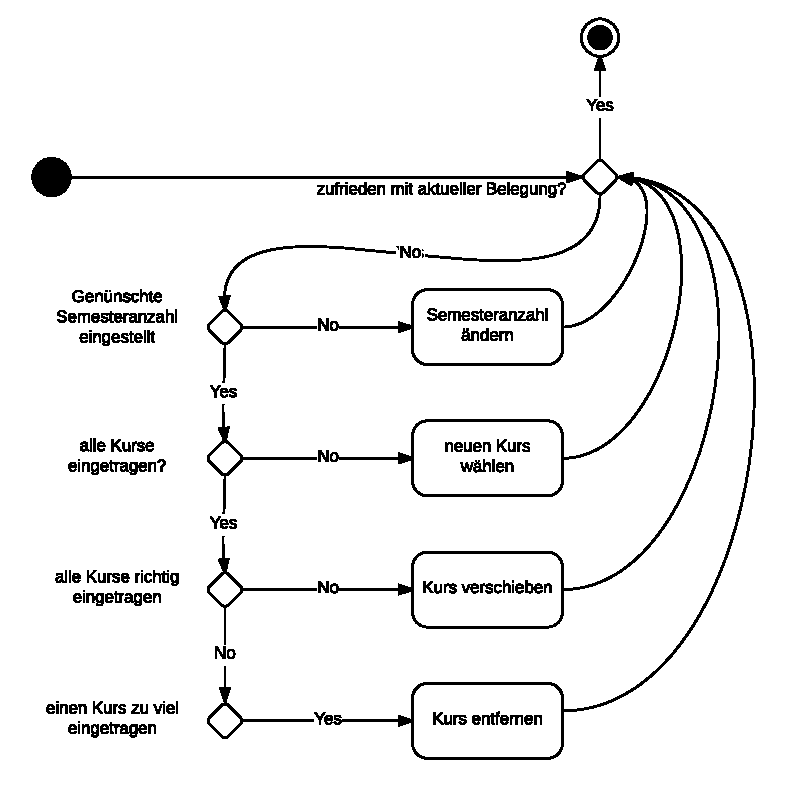
\includegraphics[width=0.8\textwidth]{figures/180_Belegungaendern_aktivitaet.pdf}
\caption{Aktivitätsdiagram vom Use Case Belegung wählen}
\label{fig:aktivity_belegung_waehlen}
\end{figure}

\begin{figure}[h!]
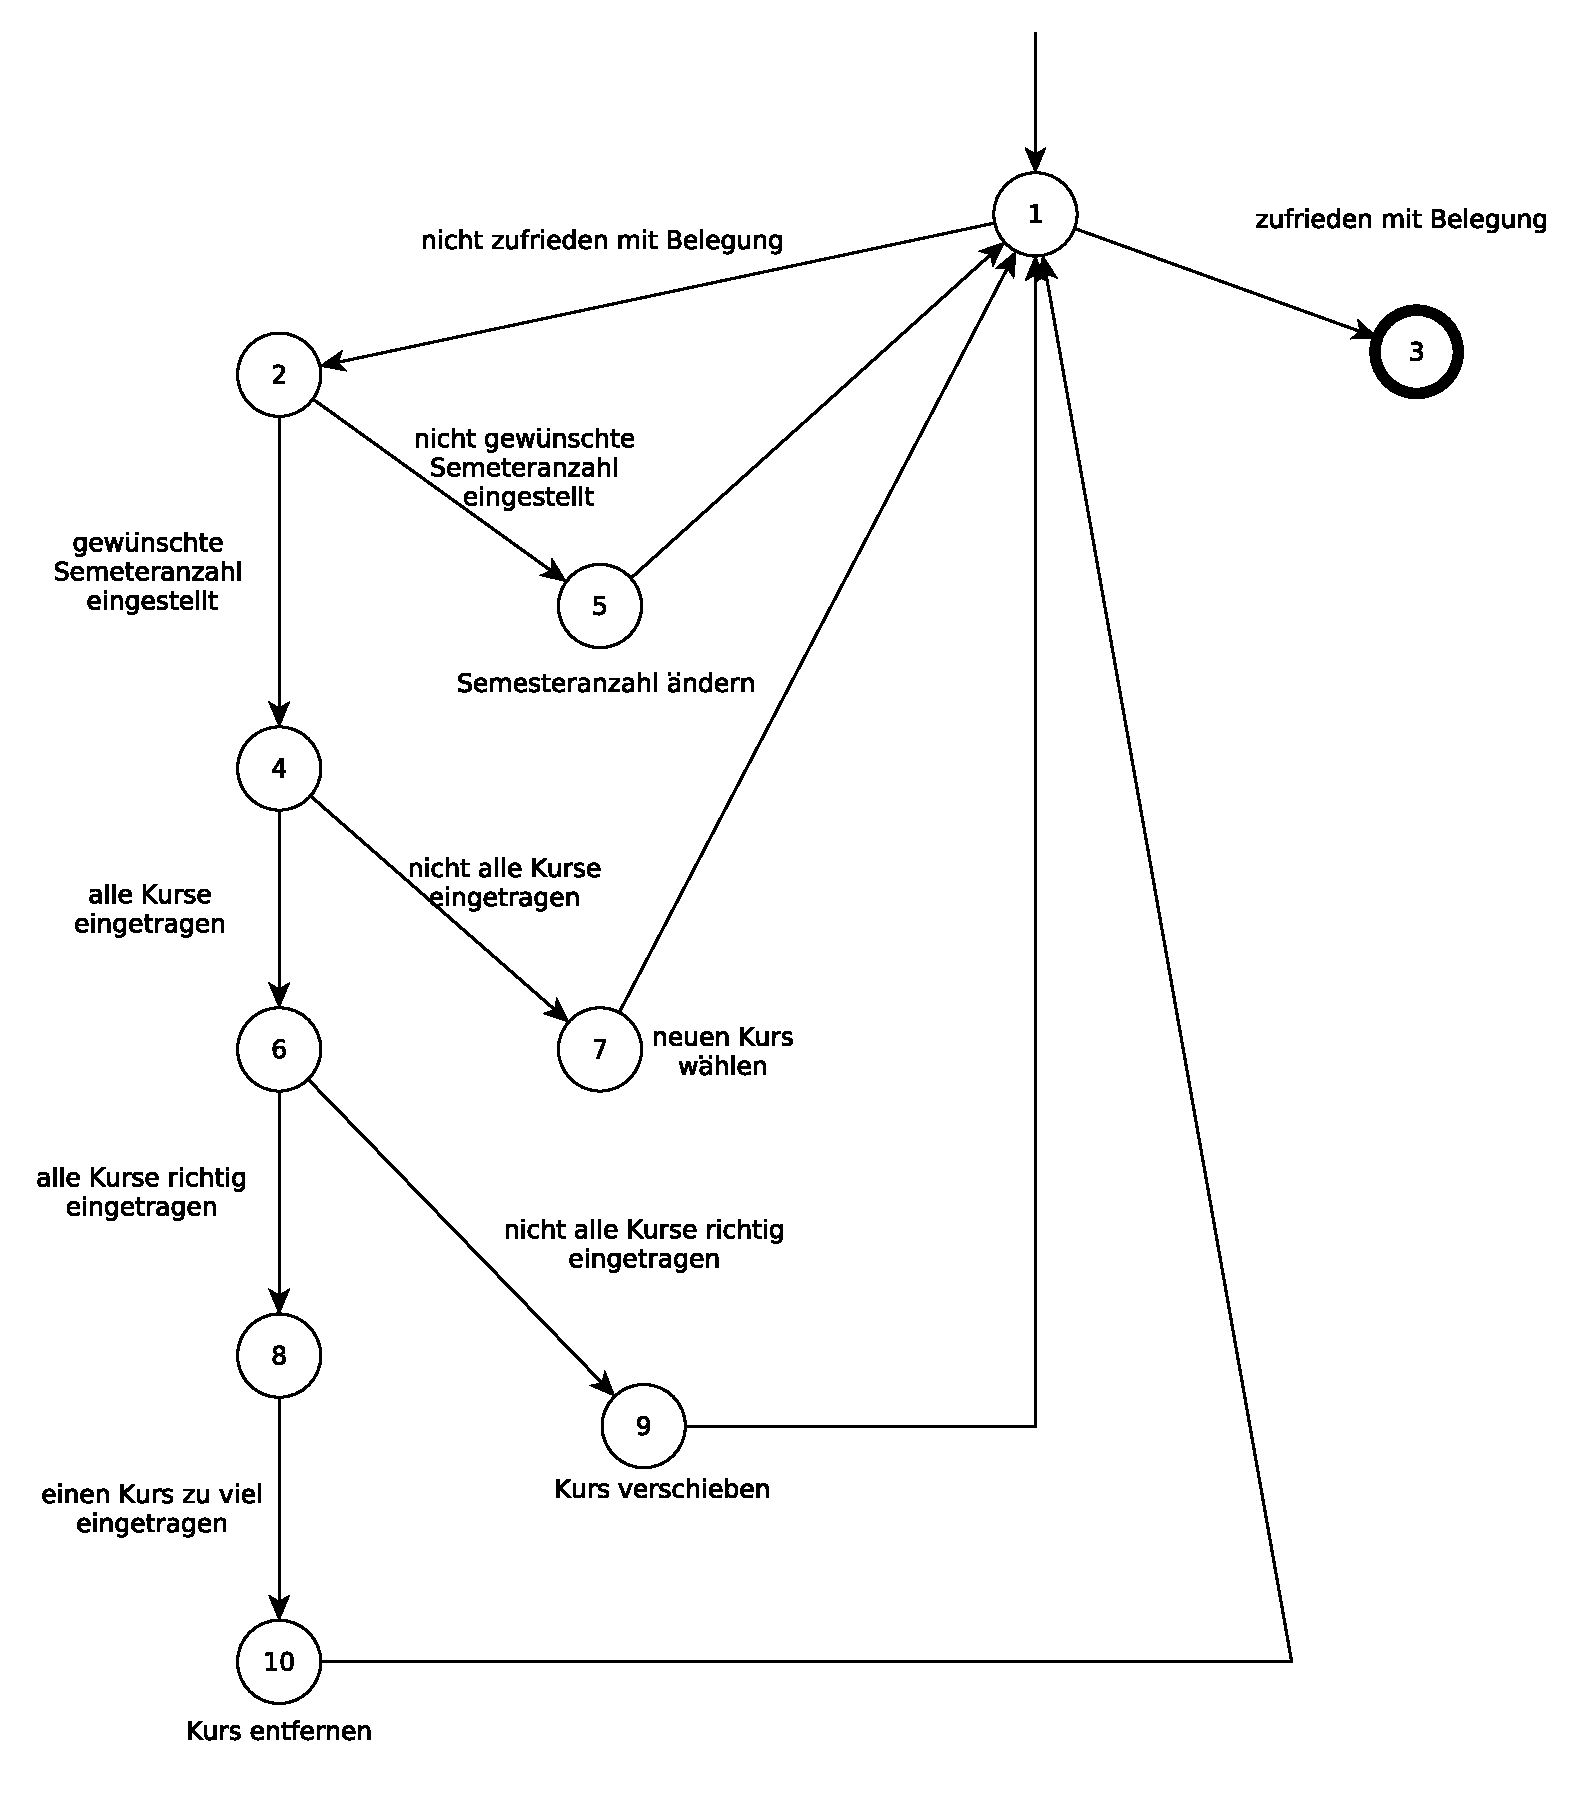
\includegraphics[width=0.8\textwidth]{figures/belegung_waehlen_use_case.pdf}
\caption{Graph vom Use Case Belegung wählen}
\label{fig:graph_belegung_waehlen}
\end{figure}

In diesem Use Case ist es theoretisch möglich, dass ein Nutzer alle einzelnen Teile oder auch eine Auswahl davon benutzt. Im Regelfall werden die Nutzer explorativ einen Plan zusammenstellen und alle Aktionen früher oder später nacheinander ausführen.
Daher werden wir alle Pfade in einem einzigen großen Testfall abdecken, welcher alle Kanten und alle Knoten des Graphens mindestens einmal ausführt.
Es ergibt sich folgende Reihenfolge von Knoten:
\texttt{1, 2, 5, 1, 2, 4, 7, 1, 2, 4, 6, 9, 1, 2, 4, 8, 10, 1, 3}.


\subsection{Logik Coverage}

\subsubsection{Regel für Wirtschaftliche Grundlagen}
\label{sec:wirtschaft}

Die Veranstaltung Wirtschaftliche Grundlagen wurde traditionell als zwei Veranstaltungen mit jeweils 3LP durchgeführt.
Zum Wintersemester WS13/14 wurde dies geäendert, und die Veranstaltung wurde fortan als eine Veranstaltung mit 6LP angeboten.
Da 180 unabhängig vom Jahrgang funktionieren soll, gibt es daher zwei mögliche gültige Belegungen: entweder man belegt beide 3LP Veranstaltungen oder eine 6LP Veranstaltung.
Die entsprechende Bedingung ist in Listing~\ref{lst:wirtschaft} zu sehen.

Wir wollen im Folgenden diese Regel mit \emph{Correlated Active Clause Coverage (CaCC)} abdecken.
Wir wissen, dass man in einem solchen auch einfach \emph{Combinatorial Coverage} durchführen kann, indem man alle $2^n = 2^3 = 8$ mögliche Belegungen manuell prüft.
Wir werden allerdings hier zur Übung dennoch \emph{CaCC} testen.
Vereinfacht stellen wir die Formel als $(a \land b) \lor c$ dar.
\begin{lstlisting}[caption=Wirtschafts-Regel,label={lst:wirtschaft},frame=single]
return (selectedWirtschaftI && selectedWirtschaftII) ||
        selectedWirtschaftI_II;
\end{lstlisting}

\begin{table}[h!]
\begin{tabular}{|l|l|l|l|l|l|l|l|}
\hline
\textbf{Row \#} & \textbf{a} & \textbf{b} & \textbf{c} & \textbf{P} & \textbf{$P_a$} & \textbf{$P_b$} & \textbf{$P_c$} \\
\hline \hline
 1              & T          & T          & T          & \textbf{T} &                &                &                \\
 2              & T          & T          & F          & \textbf{T} & T              &   T            &                \\
 3              & T          & F          & T          & \textbf{T} &                &                & T              \\
 4              & T          & F          & F          & \textbf{F} &                &   T            & T              \\
 5              & F          & T          & T          & \textbf{T} &                &                & T              \\
 6              & F          & T          & F          & \textbf{F} & T              &                & T              \\
 7              & F          & F          & T          & \textbf{T} &                &                & T              \\
 8              & F          & F          & F          & \textbf{F} &                &                & T              \\
 \hline
\end{tabular}
\caption{Wahrheitstabelle für Wirtschaftsregel}
\end{table}

Es ergeben sich folgende Fälle, in denen die Variablen jeweils aktiv werden:
\begin{align}
    P_a &= \{ (2, 6) \} \\
    P_b &= \{ (2, 4) \} \\
    P_c &= \{ 3, 5, 7 \} \times \{ 4, 6, 8 \}
\end{align}
Mit den Test Paths $TP = \{ 2, 3, 4, 6 \}$ decken wir alle Klauseln ab\footnote{Tests siehe \url{https://github.com/knub/onehundredandeighty/blob/testing/test/wirtschafts_rule_coverage.js}}.
Dies ist gleichzeitig auch die kleinste Menge die \emph{CaCC} erreicht.

\subsubsection{Regeln für Vertiefungsgebiete}
\label{sec:vertiefungsgebiete}

Die Regeln für Vertiefungsgebiete sind der komplizierteste Teil der Studienordnung.
\begin{quote}
    \begin{displayquote}
Die Modulgruppen ``Vertiefungsgebiet 1'' (VT1) und ``Vertiefungsgebiet 2'' (VT2) verfolgen die vertiefende Beschäftigung mit fachwissenschaftliche Themen des IT-Systems Engineering.
Es werden die folgenden Vertiefungsgebiete angeboten:
\begin{itemize}
    \item \emph{BPET}: Business Process \& Enterprise Technologies
    \item \emph{HCT}: Human Computer Interaction \& Computer Graphics Technology
    \item \emph{IST}: Internet \& Security Technology
    \item \emph{OSIS}: Operating Systems \& Information Systems Technology
    \item \emph{SAMT}: Software Architecture \& Modeling Technology
\end{itemize}
Es sind Module in zwei Vertiefungsgebieten in einem Gesamtumfang von 24 LP zu absolvieren, wobei in VT1
bzw. VT2 jeweils mindestens 9 LP zu erbringen sind. In VT1 und VT2 müssen mindestens je eine Vorlesung
(VT1-V und VT2-V) im Umfang von 6 LP erbracht werden. Weiter müssen ergänzende Lehrveranstaltungen
(VT1-E, VT2-E, VT1/2-E) im Umfang von 12 LP absolviert werden, die sich auf beide Vertiefungsgebiete in
den möglichen Kombinationen 3+9 LP, 6+6 LP oder 9+3 LP verteilen.
    \end{displayquote}
    \captionof{floatquote}{§~9 (3) der Studienordnung}
    \label{quo:vertiefungsgebiete}
\end{quote}
Diese Regel kann man als eine große Konjunktion der folgenden logischen Ausdrücke sehen:
\begin{itemize}
    \item $a = \text{Mind. zwei Vertiefungsgebiete (VG) sind belegt}$
    \item $b = \text{Mind. 24 LP wurden in VGs belegt}$.
    \item $c = \text{Mind. 9 LP pro VG wurden erbracht}$.
    \item $d = \text{Mind. 1 Vorlesung mit 6LP wurde pro VG erbracht}$.
\end{itemize}
Der letzte Satz der Regel folgt aus den vorhergehenden Regeln.
Damit ergibt sich als Formel $a \land b \land c \land d$ dar.
Wir wollen im Folgenden diese Regel mit \emph{Correlated Active Clause Coverage (CaCC)} abdecken.
Für CaCC für solch eine Konjunktion zu erreichen, müssen alle Variablen auf \emph{true} gesetzt werden, und die jeweils zu testende aktive Variable auf \emph{true} sowie auf \emph{false} gesetzt.
Das Problem ist allerdings, dass die Regeln teilweise aufeinander aufbauen, und dies deswegen nicht immer möglich ist.
In \emph{onehundredandeighty} werden diese Regeln allerdings nacheinander geprüft und es wird jeweils mit einer entsprechenden Fehlermeldung abgebrochen.
Wir werden also im Folgenden pro Klausel zwei Testfälle entwickeln, einmal ist die Klausur \emph{true} und einmal \emph{false}, und dann jeweils auf die korrekte Fehlermeldung überprüfen.

\textbf{Testfälle:}\footnote{\url{https://github.com/knub/onehundredandeighty/blob/testing/test/vertiefungsgebiete_coverage.js}} \\
\begin{itemize}
    \item \emph{Klausel a}
        ``Es werden nur Veranstaltungen des VG OSIS belegt'' vs. ``Es werden Veranstaltungen der VG OSIS und BPET belegt''.
    \item \emph{Klausel b}
        ``Es werden nur Veranstaltungen im Umfang von 21 LP belegt'' vs. ``Es werden Veranstaltungen im Umfang von 24 LP belegt''.
    \item \emph{Klausel c}
        ``Es werden zwei VGs belegt, allerdings ein VG nur mit 6 LP'' vs. ``Es werden Veranstaltungen zweier VG mit 9 LP belegt''.
    \item \emph{Klausel d}
        ``Ein VG wird ohne Vorlesung belegt'' vs. ``Es werden beide VG mit einer VG belegt''.
\end{itemize}

Mit dieser Menge an Testpfaden spielt jede Bedingung einmal eine aktive Rolle.

Die Anwendung der Logic Coverage ist für \emph{onehundredandeighty} sinnvoll. Es gibt viele Regeln welche richtig geprüft werden müssen. Allerdings sind die meisten Regeln mit einem "Und" verbunden, so dass es keine komplizierteren zu prüfenden Klauseln gibt.

\subsection{Input}
Der Input kann von Methoden, Modulen und dem ganzen System getestet werden.
Das System hat als Input ganze Belegungspläne.
Diese sind sehr verschieden und können sehr komplex ausfallen.
Diese werden hier nicht weiter betrachtet, könnten aber eine interessante Prüfung des kompletten Eingabebereiches sein.

Es gibt in 180 Helfermethoden, welche in vielen Programmteilen benötigt werden. Eine Methode ist die \emph{cartesianProduct}-Methode, welche das kartesische Produkt zweier Mengen berechnet.
Die Methode wird sehr häufig aufgerufen, und zwar wenn es um die Berechnung der Vertiefungsgebiete geht.
Wenn Kurs A mit den Vertiefungsgebieten 1 und 3 belegt werden kann, und Kurs B mit Vertiefungsgebieten 2 und 3 entstehen daraus vier mögliche Belegungen, nämlich: \\
$\{ (\text{A als VT1}, \text{B als VT2}), (\text{A als VT1}, \text{B als VT3}), (\text{A als VT3}, \text{B als VT2}),$ \\ $(\text{A als VT3}, \text{B als VT3}) \}$.
Genau diese Varianten berechnet das kartesische Produkt.

Für diese Methode werden wir nun beispielhaft den Input testen.
Als Eingabe werden 2 Arrays erwartet, welche jeweils eine Menge darstellen.

Wir haben uns für eine Partitionierung nach der Größe der Inputarrays ent\-schie\-den.
Dabei haben wir versucht die Randfälle wie keine Elemente oder nur 1 Element eine Partition zu widmen, da diese oftmals zu Fehler führen.
Im Folgenden sind alle Partitionen dargestellt, wobei \emph{$|A1|$} die Größe vom ersten Inputarray und \emph{$|A2|$} die Größe vom zweiten Inputarray darstellt.
\begin{itemize}
\item $|A1|$ undefined und $|A2|$ undefined
\item $|A1| \geq$ 0 und $|A2|$ = undefined
\item $|A1|$ undefined und $|A2| \geq$ 0
\item $|A1|$ = 0 und $|A2|$ = 0
\item $|A1|$ = 1 und $|A2|$ = 0
\item $|A1| \geq$ 2 und $|A2|$ = 0
\item $|A1|$ = 0 und $|A2|$ = 1
\item $|A1|$ = 1 und $|A2|$ = 1
\item $|A1| \geq$ 2 und $|A2|$ = 1
\item $|A1|$ = 0 und $|A2| \geq$ 2
\item $|A1|$ = 1 und $|A2| \geq$  2
\item $|A1| \geq 2$ und $|A2| \geq $ 2
\end{itemize}

Diese Partitionierung erfüllt die Kriterien für eine gültige Partitionierung zum Inputtesten, indem sie paarweise disjunkt sind und zusammen alle möglichen Eingaben der Methode abbilden.
Andere Partitionierungen, wie zum Beispiel die Reihenfolge der Elemente haben wir nicht betrachtet, da die Reihenfolge überhaupt keine Rolle spielt.
Die entsprechenden Tests für ein Beispiel aus jeder Partition wurden implementiert \footnote{https://github.com/knub/onehundredandeighty/blob/testing/test/input.js}.

\subsection{Mutation Coverage}
Wir haben mit Hilfe von \emph{grunt-mutation-testing} \footnote{https://www.npmjs.com/package/grunt-mutation-testing} die Mutation Coverage der von uns geschriebenen Tests ermittelt.
Dabei haben wurde die Coverage von 0~\% auf 45~\% gesteigert (siehe Abbildung~\ref{fig:mutation}).
Das von uns verwendete Tool \texttt{grunt-mutation-testing} bietet folgende Mutationen an: Austauschen/Ver\-än\-dern von arithmetischen, logischen oder Vergleichs-Operatoren, Entfernen von Elementen eines Arrays, Entfernen von Statements, Verändern von Funktionsparamtern, Ändern von Literalen, sowie das Entfernen von Eigenschaften eines Objektes.
Wir haben alle diese Mutationsarten angewandt.
Dabei kann man sehen, dass einige Methoden schon fast vollständig abgedeckt sind, andere Methoden hingegen noch gar nicht getestet werden.
In vielen Methoden sind einzelne Vergleiche (z.B. $<$ kann mit $\leq$ ersetzt werden) nicht vollständing abgedeckt.

\begin{figure}[h!]
\centering
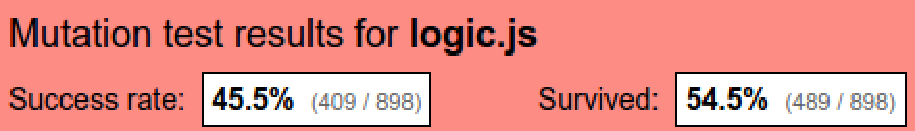
\includegraphics[width=0.5\textwidth]{figures/mutation_tests.pdf}
\caption{Ergebnisse der Mutations-Tests mit \texttt{grunt-mutation-testing}: Es wurden direkt 45 \% aller Mutanten getötet.}
\label{fig:mutation}
\end{figure}

Das Ergebnis zeigt, dass die vorher angewandten Testmethoden gut funktionieren. Besonders die Methoden für welche die Testpfade und Requirements mit Hilfe einer vorgestellten Methode entwickelt und dann umgesetzt wurden, töten sehr viele Mutanten. Somit hilft Mutation Coverage auch zu zeigen, bei welchen Programmteilen weitere Testmethoden angewandt werden sollten.


\section{Statische Analyse}

Es existieren eine Vielzahl von Tools zur statischen Analyse von JavaScript Code.
Wir haben uns 3 Tools angeschaut, die sich auf die statische Analyse spezialisiert haben: \emph{JSLint}, \emph{JSHint} und \emph{ESLint}.
Desweiteren haben wir uns den \emph{Google Closure Compiler} angeschaut, welcher keine klassische statische Analyse durchführt, allerdings trotzdem für diesen Zweck verwendet werden kann.

Bisher wurde im Projekt keine statische Analyse automatisiert in den Entwicklungsprozess eingeführt.
Allerdings wurde der Code bei der Entwicklung sporadisch manuell getestet, indem er online auf \url{http://jslint.com/} kopiert wurde.
Wie bereits erwähnt, geschah dies allerdings nicht systematisch.

Eine automatische statische Analyse hätte bereits einmal einen Fehler verhindern können.
Wie bereits weiter oben erwähnt, wurde Mitte 2014 ein Issue\footnote{\url{https://github.com/knub/onehundredandeighty/issues/20}} gemeldet, der von allen vier oben erwähnten Tools entdeckt worden wäre.
Durch die Integration dieser Tools erhoffen wir uns also insbesondere in der oft aktualisierten Datendatei \texttt{data.js} eine bessere und schnellere Erkennung von Fehlern.

\subsection{Ergebnisse der statischen Analyse}
\subsubsection{JSLint, JSHint und ESLint}
Wie bereits erwähnt sind diese drei Tools klassische Tools der statischen Analyse.
Wir werden im Folgenden eine Zusammenstellung der von den Tools gefunden Fehler präsentieren.

\begin{table}[h!]
\begin{tabular}{|l|l|c|}
\hline
\textbf{Fehler} & \textbf{Problem} & \textbf{Nr. of occurrences} \\
\hline \hline
I    & \texttt{\emph{var} ist bereits definiert}            & 17          \\
II   & \texttt{Benutze besser die Punkt-Schreibweise}       & 11          \\
III  & \texttt{Semikolon fehlt}                             & 6          \\
IV   & \texttt{Überflüssiges Semikolon}                     & 3          \\
V    & \texttt{Benutze die Funktions-Form von "use strict"} & 3          \\
VI   & \texttt{Definiere keine Funktionen in Schleifen}     & 1          \\
VII  & \texttt{Benutze !== um auf 0 zu prüfen}              & 1          \\
\hline
     &                                                      & \textbf{42 insgesamt} \\
\hline
\hline
\end{tabular}
\caption{Zusammenfassung der von den Analyse-Tools gemeldeten Fehler}
\end{table}

\paragraph{\texttt{Fehler I: Bereits definierte Variablen.}}
Diesen Fehler haben wir in 16 der 17 Fälle ignoriert, weil die Regel weitgehend interpretiert wird.
Enthält eine Methode zwei Schleifen, in denen in beiden Fällen die gleiche Schleifenvariable verwendet wird, wird ein Fehler geworfen.
Da \texttt{i} eine gängige Schleifenvariable ist, sehr oft verwendet wird und daher den Code besser lesbar macht als künstlich eingeführte andere Buchstaben, haben wir diese Regel in diesen Fällen ignoriert.
In einem Fall wurde allerdings wirklich eine Variable an einer späteren Stelle überschrieben, und mit einer neuen Bedeutung neu eingeführt.
Hier hat das Tool geholfen.

\paragraph{\texttt{Fehler II, III und IV:}}
Diese Fehler bemängeln von der typischen JavaScript Konvention abweichende Notationen und Semikolons an falschen Ständen.
Dies führt nicht direkt zu Fehlern, aber im Sinne der Lesbarkeit und Konsistenz wurden diese Fehler behoben.

\paragraph{\texttt{Fehler V: Benutze die Funktions-Form von "use strict"}}
Schreibt man an den Anfang einer JavaScript-Datei einer Datei oder Funktion den String "use strict", wird ein strengerer JavaScript-Modus angestellt, der weniger Fehler durchgehen lässt und damit ein saubereres Programmieren erzwingt.
Aus eben diesen Gründen wurde dieser Modus bei der Entwicklung gewählt.
Da das Schreiben an den Anfang der Datei Probleme verursachen kann, wenn Dateien aneinander gehangen werden (und somit der strikte Modus für alle Dateien aktiviert wird), wird empfohlen, ihn nur für bestimmte Funktionen zu aktivieren \footnote{siehe \url{https://jslinterrors.com/use-the-function-form-of-use-strict}}).
Dieses Problem besteht allerdings bei 180 nicht, da alle verwendeten Bibliotheken ebenfalls den strikten Modus verwenden, und Dateien auch nicht aneinandergehangen werden.
Daher ignorieren wir diese Meldung.

\paragraph{\texttt{Fehler VI: Definiere keine Funktionen in Schleifen}}
In der be\-män\-gel\-ten Code-Stelle, siehe Listing \ref{lst:error_6}, wurde eine Funktion innerhalb einer Schleife definiert.
Dies ist nicht gut, da in JavaScript die Funktion nicht nur einmal definiert wird, sondern wirklich in jedem Schleifendurchlauf eine neue Funktion mit identischem Code erzeugt wird.
Desweiteren kann es zu unerwarteten Seiteneffekten zwischen den Funktionen kommen \footnote{siehe \url{https://jslinterrors.com/dont-make-functions-within-a-loop}}.

\begin{lstlisting}[caption=Funktion zum Löschen von Semestern,numbers=left,label={lst:error_6},frame=single]
// removes `number` semesters from the selection,
// e.g. if number = 2 and there initially were 8 semesters
// to choose from, then there are only 6 left
removeSemester: function(number) {
  for (var i = 0; i < number; i += 1) {
    var num = semesterManager.numberDisplayed;
    $("#semester" + num).find("li").each(function() {
      /* .. Remove list element li from the web page .. */
    });
    $("#semester" + num).remove();
    semesterManager.numberDisplayed -= 1;
  }
}
\end{lstlisting}

Dementsprechend haben wir dieses Problem behoben, indem wir die Funktion als eigenständige Funktion ausgelagert haben.
Die betreffende Codezeile 7 liest sich nach der Änderung wie folgt:
\texttt{[...].each(removeListFromSemester);}

\paragraph{\texttt{Behler VII: Benutze !== um auf 0 zu prüfen}}

Dies ist ein typischer Fehler in JavaScript, der zu schwer zu debuggenden Programmen führen kann.
JavaScript zwischen zwei Vergleichsoperatoren == (!=) und === (!==).
Ersterer führt vor der Gleichheit eventuell Typumwandlungen um, um die beiden Operanden vergleichbar zu machen.
Das führt zu mitunter merkwürdigen Ergebnissen, wie Abbildung \ref{fig:javascript_truth_table} zeigt.

\begin{figure}[h!]
\centering
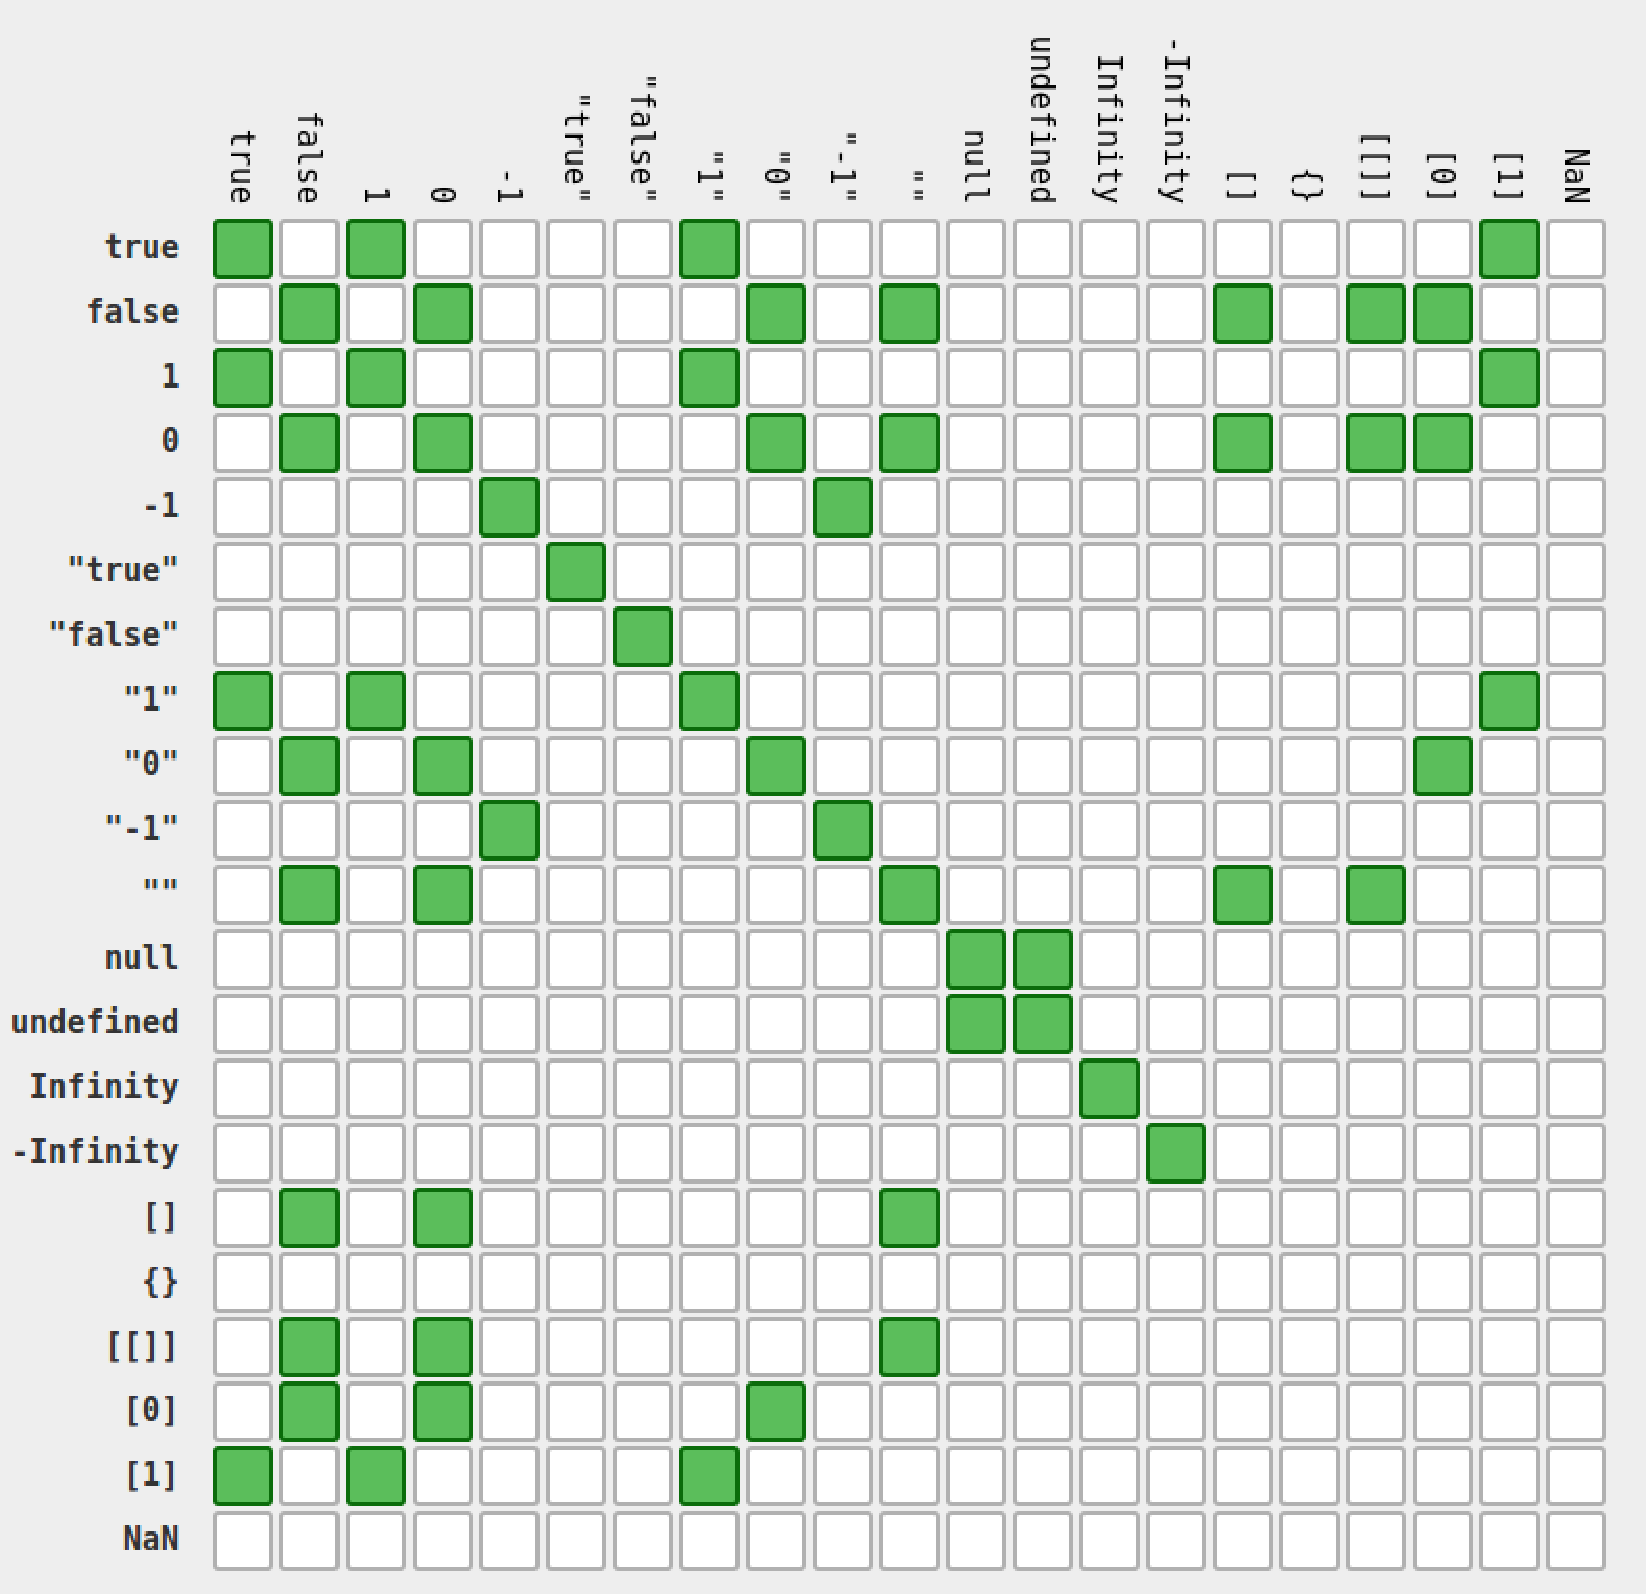
\includegraphics[width=0.8\textwidth]{figures/javascript_truth_table.pdf}
\caption{JavaScript Wahrheitstabelle: Bei Prüfung mit == sind zum Beispiel die Werte \texttt{0} (Zahl Null) und \texttt{[[]]} (ein Array, welches ein leeres Array enthält) identisch. Um solchen Unwägbarkeiten zu entgehen, sollte man immer mit === prüfen, welches keine Typ-Umwandlungen durchführt.}
\label{fig:javascript_truth_table}
\end{figure}

Dieser Fall ist leicht zu beheben, indem einfach === verwendet wird.

Alle hier verwendeten Analyse-Tools sind eher pessimistisch, da sie auch nur potentielle Fehler wie zum Beispiel der vorgestellte Fehler V, erkennen. Ob sich nur pessimistisch sind können wir nicht sagen, da es unserer Meinung vielleicht auch sein kann, dass sie nicht alle Fehler finden.

\subsubsection{Google Closure Compiler}
Der \emph{Google Closure Compiler} ist kein klassisches Code Analyse Tool.
Die eigentliche Funktion des Tools ist es, JavaScript Code so zu kompilieren, dass er schneller herunterlad- und ausführbar ist.
Dieses Kompilieren benutzt allerdings auch eine statische Analyse, welche analysiert, zu welchen Browser-Versionen das JavaScript kompatibel ist.
Wir haben dieses Teil benutzt um unsere Anwendung überprüfen zu lassen.
Dabei kam heraus, dass die Anwendung nicht kompatibel zum Internet Explorer 8 oder älter geschrieben wurde, da inkompatibles JavaScript verwendet wird.
Neuere Versionen stellen allerdings kein Problem dar.
Wir haben dies nicht weiter verfolgt, da wir keine solch alten Versionen unterstützen möchten.
Das Tool arbeitet mit \emph{optimistic inaccuracy}, d.h. wenn eine Meldung auftritt, wissen wir, dass es ein Problem gibt.
Aus der Tatsache, dass für andere Browser keine Fehler gemeldet wurden, können wir aber nicht schließen, dass 180 auf diesen problemlos läuft.

\subsubsection{Domänenspezifische Analyse für \texttt{data.js}}
Wie bereits erwähnt ist das Hauptproblem in der Wartungsphase die Änderungen an \texttt{data.js}, die in jedem Semester vorgenommen werden müssen.
Hierfür bietet sich eine domänenspezifische Analyse an, die immer bei Änderungen an der Datei durchgeführt wird.
Diese kann als Plausibilitätsprüfung verstanden werden.
In folgenden Fällen ist ein Fehler zum Beispiel wahrscheinlich:
\begin{itemize}
    \item Ein Professor bietet eine Vorlesung in einem fachfremden Vertiefungsgebiet an.
    \item Es gibt einen Rechtschreibfehler im Namen einer Veranstaltung
    \item Veranstaltungen haben weniger als zwei oder mehr als drei Vertiefungsgebiete
\end{itemize}
Das Tool würde mit \emph{pessimistic inaccuracy} arbeiten, da nicht jeder Fehler wirklich ein Fehler sein muss.

\subsubsection{Einbindung in den Entwicklungsprozess}
Nach Testen aller Tools haben wir uns entschieden, JSHint und ESLint automatisiert in den Entwicklungsprozess zu integrieren.
Diese Integration beinhaltet eine fertige Konfiguration der zu testenden Regeln und Dateien.
Eine weitere Integration von JSLint wurde nicht durchgeführt, da die beiden erst genannten Projekte besser nutzbar sind und bereits alle statischen Analysemöglichkeiten abdecken.
Die statische Analyse kann nun automatisch mit dem Befehl \texttt{grunt jshint} bzw. \texttt{eslint js/} aus dem Root-Verzeichnis des Repositories gestartet werden.

\section{Verifikation}

\subsection{Symbolic Execution}
Für Javascript gibt es leider kein Tool zur symbolischen Ausführung des Codes.
Es existiert zwar ein Paper ``A Symbolic Execution Framework for JavaScript'' mit vielen Zitierungen, das zugehörige Tool Kudzu konnten wir aber nicht online finden.

Unter der Annahme, dass ein entsprechendes Code-Verifikations-Tool existiert, haben wir im Folgenden einen Teil unseres Codes identifiziert, den wir verifizieren würden.
Es handelt sich um den komplexesten Teil des Codes, die Verifizierung der Vertiefungsgebiete, die insgesamt über 350 Zeilen einnimmt.
Die Überprüfung erfolgt schrittweise, indem zunächst das Kreuzprodukt aller möglichen Belegungen gebildet wird, und dann Schritt für Schritt ungültige Kombinationen ausgefiltert werden.
Listing~\ref{lst:vertiefung} zeigt den Algorithmus in Pseudo-Code.

\begin{lstlisting}[caption=Pseudo-Code zur Prüfung von Vertiefungsgebieten,numbers=left,label={lst:vertiefung},frame=single]
function checkSpecialisationArea(chosenCourses) {
    var cp = cartesianProduct(chosenCourses);
    cp = filter24CP(cp);
    cp = filterHaveTwoSpecialisationAreas(cp);
    cp = cleanup(cp);
    cp = haveLecture(cp);
}
\end{lstlisting}

Der Aufbau der Methode erlaubt es, für die einzelnen Schritt gute Vor- und Nachbedingungen angegeben, die automatisch überprüft werden können.
\begin{itemize}
    \item
        \textbf{Zeile 2:} \\
        Vorbedingung: \texttt{chosenCourses} ist eine Liste der vom Nutzer gewählten Kurse, zusammen mit den möglichen Vertiefungsgebieten dieser Kurse
        Nachbedingung: \texttt{cp} enthält das kartesische Produkt der Belegungen
    \item
        \textbf{Zeile 3:} \\
        Nachbedingung: Keine der Kombination in \texttt{cp} enthält eine Kombination, in der weniger als 24 LP gewählt wurden.
    \item
        \textbf{Zeile 4:} \\
        Nachbedingung: Alle Kombinationen in \texttt{cp} enthalten genug Kurse, um die LP-Anforderungen für zwei Vertiefungsgebiete zu erfüllen.
    \item
        \textbf{Zeile 5:} \\
        Nachbedingung: \texttt{cp} enthält keine Duplikate und auch keine Belegungen, die Teilmengen anderer in \texttt{cp} enthaltenen Belegungen sind.
    \item
        \textbf{Zeile 6:} \\
        Nachbedingung: \texttt{cp} enthält mind. eine Vorlesung für alle Paare von Vertiefungsgebieten aus Zeile 4
\end{itemize}
Der Aufbau der Listen funktioniert in allen Schritten so, dass eine neue, leere Liste angelegt wird, und dann schrittweise mit den Kombinationen aus dem vorigen Schritt gefüllt wird, die die neue Bedingung erfüllen.
Insofern würden sich auch gute Schleifeninvarianten ergeben.
Symbolische Ausführung würde sich für diese Methoden ebenfalls anbieten, da damit Test-Daten generiert werden könnten, die die Vertiefungsgebiete-Regel abtesten könnten.
    % // keine Belegung ist subset einer anderen gültigen Belegung


\subsection{Type Analysis}
Das Tool \emph{TAJS} (\url{http://www.brics.dk/TAJS/}) ist ein Type Analyzer für Javascript, entwickelt von Anders Møller et al.
Man kann damit Call-Graphen sehen oder auch Datenflussanalysen durchführen.

Wir haben uns verschiedene Flussgraphen der einzelnen Programme angeschaut.
In Abbildung \ref{fig:tajs} ist beispielhaft der Flussgraph der in Kapitel \ref{sec:wirtschaft} vorgestellten Wirtschaftsregel\footnote{\url{https://github.com/knub/onehundredandeighty/blob/testing/js/logic.js\#L674-L679}} zu sehen.

\begin{figure}[h!]
\centering
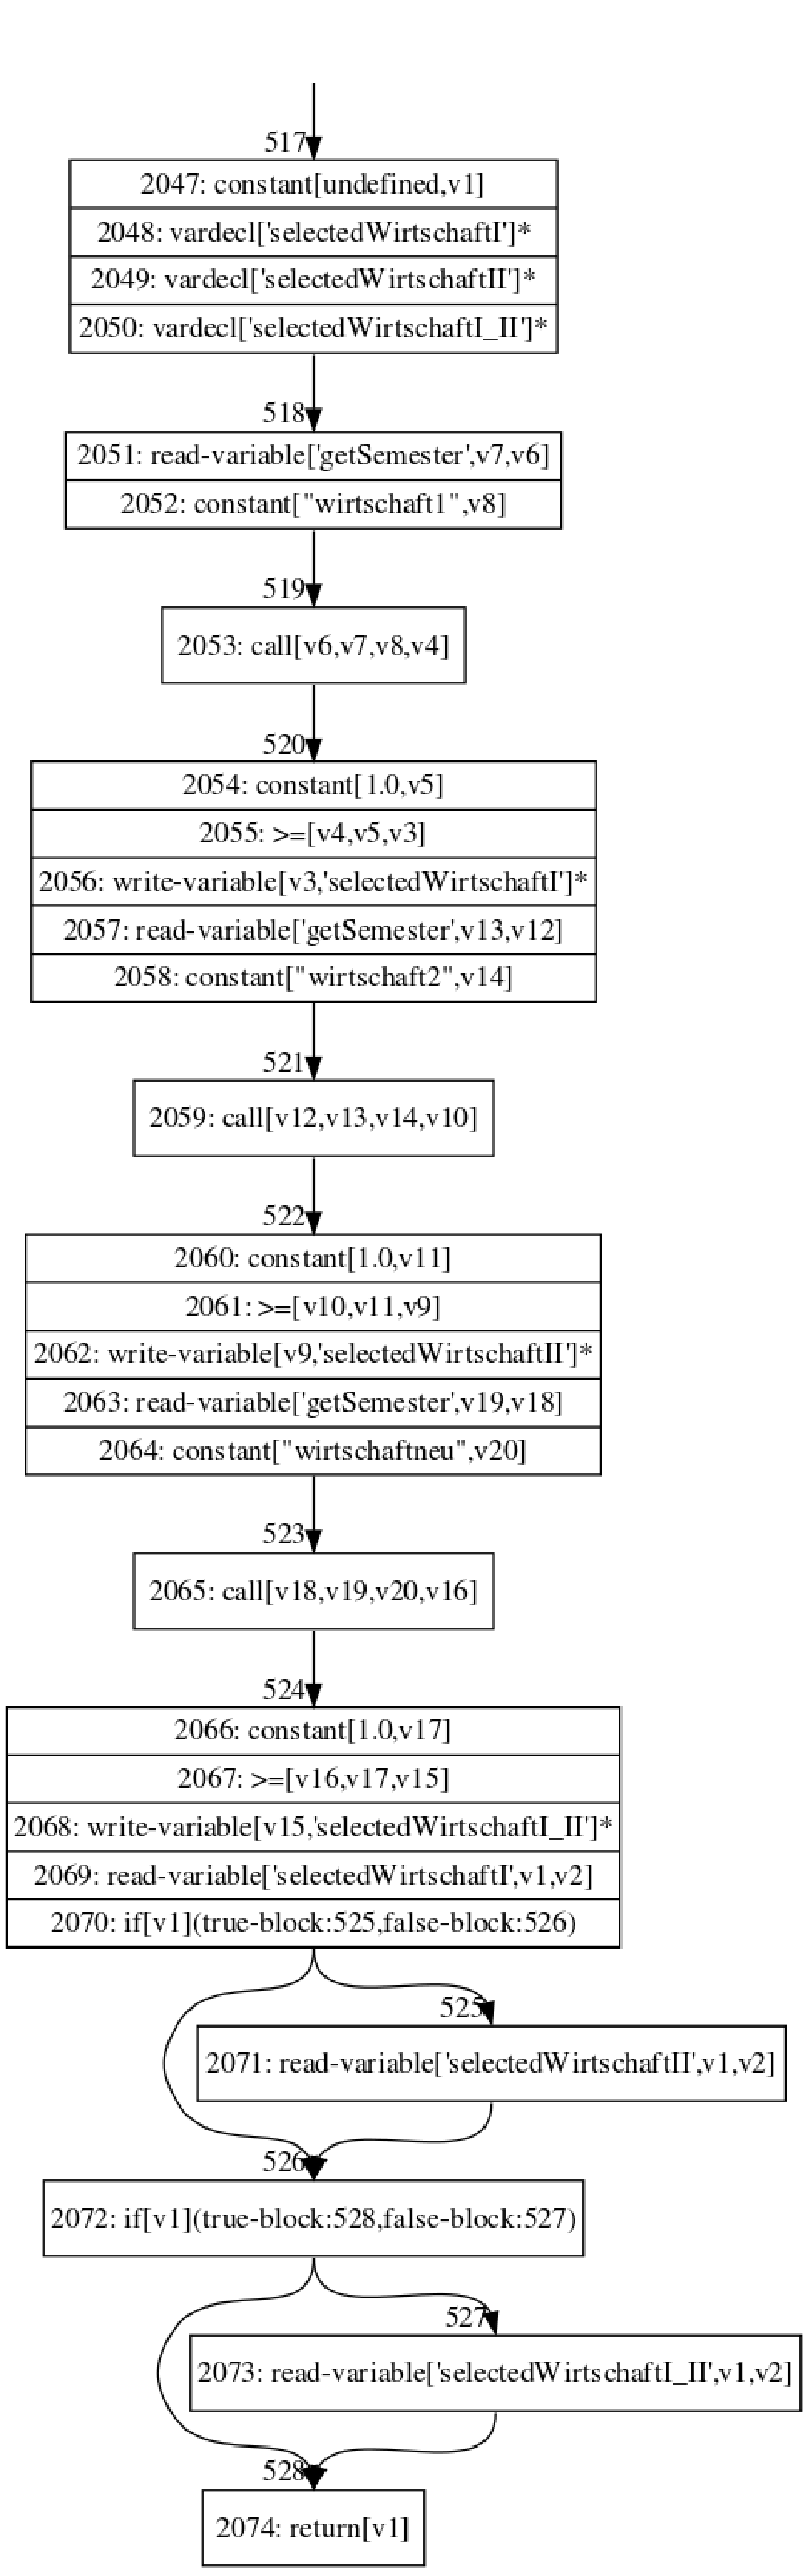
\includegraphics[width=0.5\textwidth]{figures/tajs.pdf}
\caption{Flow Graph der Wirtschaftsregel, analysiert von TAJS}
\label{fig:tajs}
\end{figure}

Man erkennt klar die Deklaration (vardecl) der einzelnen Variablen, sowie die verschiedenen Initialisierungen (write-variable) und wann eine Variable gelesen wird (read-variable).
Genauso sind verschiedene Funktionsaufrufe (\texttt{getSemester}) und Konstantendefinitionen (\texttt{Literal 1}) enthalten.
Gegen Ende der Funktion kann erkannt werden, dass Short-Circuit Operationen enthalten sind.
Diese Art von Ausgabe stellt sehr schön graphisch dar, welche Schritte die einzelnen Variablen durchlaufen.
Man erkennt auch die Short-Circuit Auswertung des logischen Ausdrucks am Ende der Funktion.
Allerdings können diese Diagramme sehr schnell sehr groß und unübersichtlich werden, so dass sie nur für die Analyse von kleinen Programmabschnitten geeignet sind.
Diese Analyse ist gleichzeitig ein Vorverarbeitungsschritt von TAJS, um die ungültige Verwendung von Variablen zu erkennen, z. B. ob sie gelesen wird bevor sie geschrieben wird oder nie verwendet wird.
Wir haben TAJS auf unser Projekt angewandt, diese Art von Fehler tritt allerdings bei 180 nicht auf.

Unser Fazit ist, dass Verifikations-Tools deutlich schwieriger einzurichten sind, als die bisher genutzten Tools.
Auch ist es nicht leicht die Ausgaben zu verstehen.
Das Kosten-Nutzen-Verhältnis hat sich in unserem Projekt nicht rentiert.
Wir würden solche Werkzeuge nur für wirklich kritischen Code nutzen, und wenn genug Einarbeitungszeit zur Verfügung steht.

\section{Zusammenfassung}

Wir haben nach Anwendung verschiedener Test-Coverage-Methoden, der Tools zur statischen Analyse sowie der Betrachtung der Verifikation keinen Bug gefunden.
Allerdings sind einige Unsauberkeiten in der Programmierung entfernt.

Beim Testen haben wir uns auf Graph Coverage an den beiden Fällen Control Flow Coverage und Use Cases konzentriert.
Diese Methoden konnten wir beispielhaft bei \emph{onehundredandeighty} an ausgewählten Programmteilen erfolgreich umsetzen.
Dabei halfen uns die Methoden dabei, die richtigen Testpfade und Requirements zu finden.
Allerdings sind die Methoden sehr aufwändig, so dass sie nicht für das ganze Programm umgesetzt wurden.
Logik Coverage haben wir an zwei verschiedenen Beispielen umgesetzt.
Dabei stellte sich heraus, dass 180 zwar viel Logik enthält, diese sich allerdings in recht einfachen bool'schen Ausdrücken umsetzen lässt (z.B. nur eine größe Konjunktion bei den Vertiefungsgebieten).
Daher konnten wir die Möglichkeiten der Logik Coverage nicht komplett ausreizen.
Desweiteren haben wir Input-Testing am Beispiel der Berechnung des kartesischen Produkts getestet.
Diese Methode war hilfreich und hat uns geholfen, ein hohes Vertrauen in das Funktionieren der Methode zu gewinnen.
Input-Testing lässt sich auch recht leicht und damit für viele Methoden anwenden.

Insgesamt haben wir die Testanzahl von 0 zu Beginn des Seminars auf 38 erhöht.
Die Mutation Coverage erreichte 45~\%.
Besonders die Methoden, welche mit bestimmten Coverage Methoden getestet wurden, konnte viele Mutanten töten.
Dies bestätigt, dass die vorgestellten und genutzten Coverage-Methoden eine gute Testabdeckung erzeugen.

Im Bereich der statischen Analyse wurden vier verschiedene Tools angewandt: JSLint, JSHint, ESlint und Google Closure Compiler.
Diese ermittelten einige Warnungen, welche allerdings nie ein externes, vom Nutzer sichtbares Fehlverhalten im Programm hervorgerufen hätten.
Sie haben eher dazu beigetragen, unseren Programmierstil sauberer zu gestalten, und damit in Zukunft vielleicht weniger neue Bugs zu erzeugen.
Von der Integration von JSHint und ESLint erhoffen wir uns allerdings, dass bereits in der Vergangenheit aufgetretene Fehler in der Syntax in Zukunft vermieden werden.
Da diese Tools mit \emph{pessimistic inaccuracy} arbeiten, und jetzt keine Fehler mehr melden, können wir davon ausgehen, dass die getesteten Fehlertypen in unserem Programm nicht auftreten.
Insgesamt sind wir mit der Nutzung der Analyse-Tools zufrieden und werden diese oder ähnliche Tools in Zukunft auch bei anderen Projekten einsetzen.
Die Schwierigkeit liegt lediglich im Aufsetzen der Tools und der Konfiguration.
Ist dies einmal geschehen, hat man eine Infrastruktur aufgebaut die ohne großen Wartungsaufwand auch in Zukunft potentielle Defekte schnell aufdecken kann.

Im Rahmen des Seminares konnten wir nur einige beispielhafte Programmteile prüfen.
Des weiteren haben wir uns nur mit der Logik beschäftigt und das Frontend außen vor gelassen.
Für gesamtheitliches Testen müssten auch die ausgelassenen Programmteile betrachtet werden.
Bei der Analyse der Anforderungen kam auch die Anforderung auf, dass mit den Daten des Nutzers verantwortlich umgegangen wird und diese den Rechner des Nutzers nie verlassen.
Diese Anforderung wurde beim Testen hier ignoriert, da wir dafür nicht die passenden Werkzeuge gefunden haben.

Abschließend kann man sagen, dass die angewandten Methoden das Programm nun deutlich besser testen und wir höheres Vertrauen in die Korrektheit der Anwendung gewinnen konnten.
Die Anwendung war allerdings schon recht gut entwickelt, sodass wir in den von uns untersuchten Teilen keine Fehler finden konnten.

\end{document}
